\documentclass[CJK,13pt]{beamer}
\usepackage{CJKutf8}
\usepackage{beamerthemesplit}
\usetheme{Malmoe}
\useoutertheme[footline=authortitle]{miniframes}
\usepackage{amsmath}
\usepackage{amssymb}
\usepackage{graphicx}
\usepackage{eufrak}
\usepackage{color}
\usepackage{slashed}
\usepackage{simplewick}
\usepackage{tikz}
\usepackage{tcolorbox}
\usepackage{ulem}
\graphicspath{{../figures/}}
%%figures
\def\lfig#1#2{\includegraphics[width=#1 in]{#2}}
\def\tfig#1#2{\includegraphics[height=#1 in]{#2}}
\def\addfig#1#2{\begin{center}\includegraphics[width=#1 in]{#2}\end{center}}
\def\question{
\includegraphics[width=0.3in]{why.jpg}\,}
\def\answer{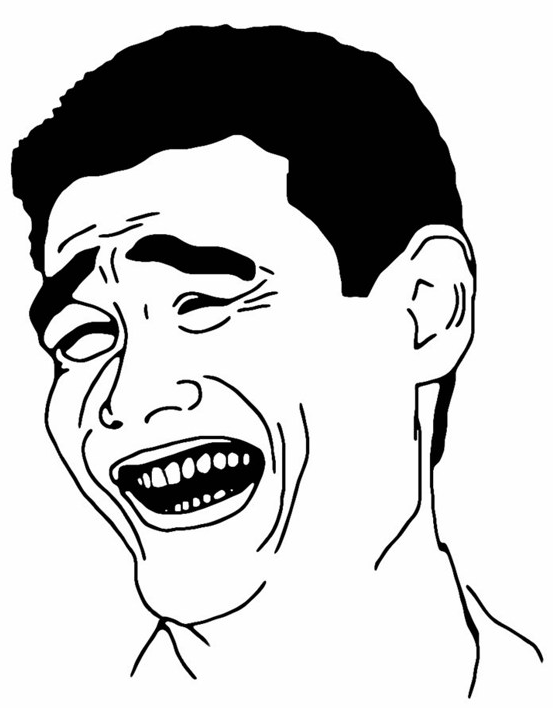
\includegraphics[width=0.3in]{baozou_haha.png}\,}
\def\wulian{
\includegraphics[width=0.18in]{emoji_wulian.jpg}}
\def\bigwulian{
\includegraphics[width=0.35in]{emoji_wulian.jpg}}
\def\bye{
\includegraphics[width=0.18in]{emoji_bye.jpg}}
\def\bigbye{
\includegraphics[width=0.35in]{emoji_bye.jpg}}
\def\huaixiao{
\includegraphics[width=0.18in]{emoji_huaixiao.jpg}}
\def\bighuaixiao{
\includegraphics[width=0.35in]{emoji_huaixiao.jpg}}
\def\jianxiao{
\includegraphics[width=0.18in]{emoji_jianxiao.jpg}}
\def\bigjianxiao{
\includegraphics[width=0.35in]{emoji_jianxiao.jpg}}
\def\haoqi{
\includegraphics[width=0.18in]{emoji_haoqi.jpg}}
%% colors
\def\blacktext#1{{\color{black}#1}}
\def\bluetext#1{{\color{blue}#1}}
\def\redtext#1{{\color{red}#1}}
\def\darkbluetext#1{{\color[rgb]{0,0.2,0.6}#1}}
\def\skybluetext#1{{\color[rgb]{0.2,0.7,1.}#1}}
\def\cyantext#1{{\color[rgb]{0.,0.5,0.5}#1}}
\def\greentext#1{{\color[rgb]{0,0.7,0.1}#1}}
\def\darkgray{\color[rgb]{0.2,0.2,0.2}}
\def\lightgray{\color[rgb]{0.6,0.6,0.6}}
\def\gray{\color[rgb]{0.4,0.4,0.4}}
\def\blue{\color{blue}}
\def\red{\color{red}}
\def\orange{\color[rgb]{1.,0.8,0.}}
\def\green{\color{green}}
\def\darkgreen{\color[rgb]{0,0.4,0.1}}
\def\darkblue{\color[rgb]{0,0.2,0.6}}
\def\skyblue{\color[rgb]{0.2,0.7,1.}}
%%control
\def\diag{\mathrm{diag}\,}
\def\heaviside{\,\mathrm{h}\,}
\def\bral{\left(\begin{array}{l}}
\def\brar{\end{array}\right)}
\def\brall{\left(\begin{array}{ll}}
\def\brarr{\end{array}\right)}
\def\bralll{\left(\begin{array}{lll}}
\def\brarrr{\end{array}\right)}
\def\branchl{\left\{\begin{array}{l}}
\def\branchr{\end{array}\right.}
\def\branchll{\left\{\begin{array}{ll}}
\def\branchrr{\end{array}\right.}
\def\branchlll{\left\{\begin{array}{lll}}
\def\branchrrr{\end{array}\right.}
\def\sfgamma#1{\,\Gamma\left( #1 \right)\,}
\def\be{\begin{equation}}
\def\ee{\nonumber\end{equation}}
\def\bea{\begin{eqnarray}}
\def\eea{\nonumber\end{eqnarray}}
\def\bch{\begin{CJK}{UTF8}{gbsn}}
\def\ech{\end{CJK}}
\def\bitem{\begin{itemize}}
\def\eitem{\end{itemize}}
\def\bcenter{\begin{center}}
\def\ecenter{\end{center}}
\def\bex{\begin{minipage}{0.2\textwidth}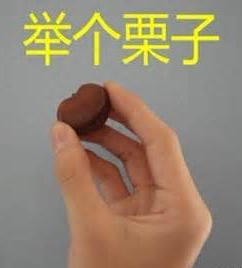
\includegraphics[width=0.6in]{jugelizi.png}\end{minipage}\begin{minipage}{0.76\textwidth}}
\def\eex{\end{minipage}}
\def\chtitle#1{\frametitle{\bch#1\ech}}
\def\bmat#1{\left(\begin{array}{#1}}
\def\emat{\end{array}\right)}
\def\bcase#1{\left\{\begin{array}{#1}}
\def\ecase{\end{array}\right.}
\def\bmini#1{\begin{minipage}{#1\textwidth}}
\def\emini{\end{minipage}}
\def\tbox#1{\begin{tcolorbox}#1\end{tcolorbox}}
\def\pfrac#1#2#3{\left(\frac{\partial #1}{\partial #2}\right)_{#3}}
\def\res#1#2{\,\mathrm{res}\,#1\left(#2\right)\,}
\def\newt#1#2{\left(\begin{array}{c}#1\\ #2\end{array}\right)}
\def\reof#1{\,\mathrm{Re}{\left(#1\right)\,}}
\def\imof#1{\,\mathrm{Im}{\left(#1\right)\,}}
\def\Arg#1{\,\mathrm{Arg}\,#1\,}
%%symbols
\def\intfull{\int_{-\infty}^\infty}
\def\inthalf{\int_0^\infty}
\def\bropt{\,(\ \ \ )}
\def\sech{\mathrm{sech}\,}
\def\csch{\mathrm{csch}\,}
\def\asinh{\mathrm{asinh}\,}
\def\acosh{\mathrm{acosh}\,}
\def\sone{$\star$}
\def\stwo{$\star\star$}
\def\sthree{$\star\star\star$}
\def\sfour{$\star\star\star\star$}
\def\sfive{$\star\star\star\star\star$}
\def\rint{{\int_\leftrightarrow}}
\def\roint{{\oint_\leftrightarrow}}
\def\stdHf{{\textit{\r H}_f}}
\def\deltaH{{\Delta \textit{\r H}}}
\def\ii{{\dot{\imath}}}
\def\skipline{{\vskip0.1in}}
\def\skiplines{{\vskip0.2in}}
\def\lagr{{\mathcal{L}}}
\def\hamil{{\mathcal{H}}}
\def\vecT{{\mathbf{T}}}
\def\vecN{{\mathbf{N}}}
\def\vecB{{\mathbf{B}}}
\def\vecv{{\mathbf{v}}}
\def\vecr{{\mathbf{r}}}
\def\vecf{{\mathbf{f}}}
\def\vecg{{\mathbf{g}}}
\def\vecupsilon{{\mathbf{\upsilon}}}
\def\vecu{{\mathbf{u}}}
\def\vecj{{\mathbf{j}}}
\def\vecx{{\mathbf{x}}}
\def\vecy{{\mathbf{y}}}
\def\vecz{{\mathbf{z}}}
\def\veck{{\mathbf{k}}}
\def\vecp{{\mathbf{p}}}
\def\vecn{{\mathbf{n}}}
\def\vecA{{\mathbf{A}}}
\def\vecP{{\mathbf{P}}}
\def\vecsigma{{\mathbf{\sigma}}}
\def\hatJn{{\hat{J_\vecn}}}
\def\hatJx{{\hat{J_x}}}
\def\hatJy{{\hat{J_y}}}
\def\hatJz{{\hat{J_z}}}
\def\hatj#1{\hat{J_{#1}}}
\def\hatphi{{\hat{\phi}}}
\def\hatq{{\hat{q}}}
\def\hatpi{{\hat{\pi}}}
\def\vel{\upsilon}
\def\Dint{{\mathcal{D}}}
\def\adag{{\hat{a}^\dagger}}
\def\bdag{{\hat{b}^\dagger}}
\def\cdag{{\hat{c}^\dagger}}
\def\ddag{{\hat{d}^\dagger}}
\def\hata{{\hat{a}}}
\def\hatb{{\hat{b}}}
\def\hatc{{\hat{c}}}
\def\hatd{{\hat{d}}}
\def\hatD{{\,\hat{D}}}
\def\hatN{{\hat{N}}}
\def\hatH{{\hat{H}}}
\def\hatp{{\hat{p}}}
\def\Fup{{F^{\mu\nu}}}
\def\Fdown{{F_{\mu\nu}}}
\def\newl{\nonumber \\}
\def\vece{\mathrm{e}}
\def\calM{{\mathcal{M}}}
\def\calT{{\mathcal{T}}}
\def\calR{{\mathcal{R}}}
\def\barpsi{\bar{\psi}}
\def\baru{\bar{u}}
\def\barv{\bar{\upsilon}}
\def\qeq{\stackrel{?}{=}}
\def\ftf{\stackrel{\mathcal{FT}}{\Longrightarrow}}
\def\ftb{\stackrel{\mathcal{FT}}{\Longleftarrow}}
\def\ftfb{\stackrel{\mathcal{FT}}{\Longleftrightarrow}}
\def\ltf{\stackrel{\mathcal{LT}}{\Longrightarrow}}
\def\ltb{\stackrel{\mathcal{LT}}{\Longleftarrow}}
\def\ltfb{\stackrel{\mathcal{LT}}{\Longleftrightarrow}}
\def\torder#1{\mathcal{T}\left(#1\right)}
\def\rorder#1{\mathcal{R}\left(#1\right)}
\def\contr#1#2{\contraction{}{#1}{}{#2}#1#2}
\def\trof#1{\mathrm{Tr}\left(#1\right)}
\def\trace{\mathrm{Tr}}
\def\comm#1{\ \ \ \left(\mathrm{used}\ #1\right)}
\def\tcomm#1{\ \ \ (\text{#1})}
\def\slp{\slashed{p}}
\def\slk{\slashed{k}}
\def\calp{{\mathfrak{p}}}
\def\veccalp{\mathbf{\mathfrak{p}}}
\def\Tthree{T_{\tiny \textcircled{3}}}
\def\pthree{p_{\tiny \textcircled{3}}}
\def\dbar{{\,\mathchar'26\mkern-12mu d}}
\def\erf{\mathrm{erf}}
\def\const{\mathrm{const.}}
\def\pheat{\pfrac p{\ln T}V}
\def\vheat{\pfrac V{\ln T}p}
%%units
\def\fdeg{{^\circ \mathrm{F}}}
\def\cdeg{^\circ \mathrm{C}}
\def\atm{\,\mathrm{atm}}
\def\angstrom{\,\text{\AA}}
\def\SIL{\,\mathrm{L}}
\def\SIkm{\,\mathrm{km}}
\def\SIyr{\,\mathrm{yr}}
\def\SIGyr{\,\mathrm{Gyr}}
\def\SIV{\,\mathrm{V}}
\def\SImV{\,\mathrm{mV}}
\def\SIeV{\,\mathrm{eV}}
\def\SIkeV{\,\mathrm{keV}}
\def\SIMeV{\,\mathrm{MeV}}
\def\SIGeV{\,\mathrm{GeV}}
\def\SIcal{\,\mathrm{cal}}
\def\SIkcal{\,\mathrm{kcal}}
\def\SImol{\,\mathrm{mol}}
\def\SIN{\,\mathrm{N}}
\def\SIHz{\,\mathrm{Hz}}
\def\SIm{\,\mathrm{m}}
\def\SIcm{\,\mathrm{cm}}
\def\SIfm{\,\mathrm{fm}}
\def\SImm{\,\mathrm{mm}}
\def\SInm{\,\mathrm{nm}}
\def\SImum{\,\mathrm{\mu m}}
\def\SIJ{\,\mathrm{J}}
\def\SIW{\,\mathrm{W}}
\def\SIkJ{\,\mathrm{kJ}}
\def\SIs{\,\mathrm{s}}
\def\SIkg{\,\mathrm{kg}}
\def\SIg{\,\mathrm{g}}
\def\SIK{\,\mathrm{K}}
\def\SImmHg{\,\mathrm{mmHg}}
\def\SIPa{\,\mathrm{Pa}}
%page
\def\secpage#1#2{\begin{frame}\bcenter{\bf \Huge #1} \ecenter \skipline \tbox{\bcenter #2 \ecenter}\end{frame}}
\def\append#1#2{\secpage{附录#1}{#2}}
\def\thinka#1{\begin{frame}\frametitle{思考题}\bcenter\lfig{0.4}{think0.jpg}  \skipline #1 \ecenter\end{frame}}
\def\thinkb#1{\begin{frame}\frametitle{思考题}\bcenter\lfig{0.5}{think1.jpg}  \skipline #1 \ecenter\end{frame}}
\def\thinkc#1{\begin{frame}\frametitle{思考题}\bcenter\lfig{0.5}{think2.jpg}  \skipline #1 \ecenter\end{frame}}
\def\thinkd#1{\begin{frame}\frametitle{思考题}\bcenter\lfig{0.5}{think3.jpg}  \skipline #1 \ecenter\end{frame}}
\def\thinke#1{\begin{frame}\frametitle{思考题}\bcenter\lfig{0.5}{think4.jpg}  \skipline #1 \ecenter\end{frame}}
\def\thinkf#1{\begin{frame}\frametitle{思考题}\bcenter\lfig{0.5}{think5.jpg}  \skipline #1 \ecenter\end{frame}}
\def\schw{ds^2 = \left(1-\frac{2GM}{r}\right)dt^2 - \left(1-\frac{2GM}{r}\right)^{-1} dr^2 - r^2\left(d\theta^2 + \sin^2\theta d\phi^2\right)}

\input{titlepage.tex}
  \date{}
  \begin{document}
  \bch
  \tpage{14}{Spherical Symmetric Metric}

  \thinkf{证明爱因斯坦方程
    $$ R_{\mu\nu}-\frac{1}{2}g_{\mu\nu}R = 8\pi GT_{\mu\nu}$$
    可以等价地写成
    $$R_{\mu\nu} = 8\pi GT_{\mu\nu} - 4\pi GT g_{\mu\nu}$$
    这里的 $T\equiv T^\rho_{\ \ \rho}$.
  }

  \begin{frame}
    本讲的任务是研究 \sout{真空中的球形火鸡} 球对称的度规

    \addfig{1}{sphericalchicken.jpg}
  \end{frame}
  
  \begin{frame}
    \frametitle{球对称的度规是指}

    三个空间转动映射的生成元都是Killing vector……

    \addfig{1.3}{shuorenhua.jpg}
    
  \end{frame}

  \begin{frame}
  \frametitle{球对称的度规是指}

  \sout{三个空间转动映射的生成元都是Killing vector……}

  \skipline
  
    可以取坐标系 $(t, r, \theta,\phi)$,使得
   {\blue $$ ds^2 = e^{2\Phi(r,t)}dt^2 - e^{-2\Psi(r, t)}dr^2 - r^2\left(d\theta^2 + \sin^2\theta d\phi^2\right)$$}
    
    
  \end{frame}

  \begin{frame}
    \frametitle{Ricci张量}
    用 sympy 代码 \url{http://zhiqihuang.top/gr/codes/spherical.py} 以及 latex 编译器导出
    {\small

\begin{eqnarray}
R_{00} &=&  e^{2 \Phi + 2 \Psi} \left[\left(\Phi_{,r}\right)^{2} +  \Phi_{,r} \Psi_{, r} + \Phi_{,r,r}+\frac{2}{r}  \Phi_{,r}\right] - \Phi_{,t} \Psi_{,t} - \left(\Psi_{,t}\right)^{2} + \Phi_{,t,t}  \nonumber \\
R_{10} &=& - \frac{2}{r} \Psi_{,t} \nonumber \\
R_{11} &=&  e^{- 2 \Phi- 2 \Psi} \left[\Phi_{,t} \Psi_{,t} +  \left(\Psi_{,t}\right)^{2} -  \Phi_{,t,t} \right]- \left(\Phi_{,r}\right)^{2} - \Phi_{,r} \Psi_{, r} - \Phi_{,r,r} - \frac{2}{r} \Psi_{, r} \nonumber \\
R_{22} &=& 1 - r e^{2 \Psi} \Phi_{,r} - r e^{2 \Psi} \Psi_{, r} - e^{2 \Psi}  \nonumber \\
R_{33} &=& R_{22} \sin^2\theta \nonumber 
\end{eqnarray}
    }
    这些方程是我们下面讨论的出发点。
  \end{frame}

  \secpage{真空中的球形……解}{$$ ds^2 = \left(1-\frac{2GM}{r}\right)d\tau^2 - \frac{1}{1-\frac{2GM}{r}} dr^2 - r^2\left(d\theta^2 +\sin^2\theta d\phi^2\right)$$}
  
  \begin{frame}
    真空中的  Einstein 方程为 $R_{\mu\nu}=0$。由 $R_{10}=0$ 立刻得到: $\Psi_{,t}=0$,即 $\Psi$ 只依赖于$r$。

    再根据 $R_{00}= R_{11}= R_{22}=0$ ($R_{33}=R_{22}\sin^2\theta$ 不需要另外考虑) 得到:
    \begin{eqnarray}
r\left[\left(\Phi_{,r}\right)^{2} +  \Phi_{,r,r}+ \Phi_{,r} \Psi_{, r}  \right] +  2\Phi_{,r}&=& 0 \label{eq:00}\\
-r \left[\left(\Phi_{,r}\right)^{2} + \Phi_{,r} \Psi_{, r} + \Phi_{,r,r}\right] - 2 \Psi_{, r} &=&0 \label{eq:11} \\
e^{-2 \Psi}- r \left(\Phi_{,r} + \Psi_{, r}\right)  - 1  &=& 0 \label{eq:22}
    \end{eqnarray}
  \end{frame}

  \begin{frame}
方程 \eqref{eq:00} + 方程 \eqref{eq:11},得到 $(\Phi - \Psi)_{,r}=0$,积分即得到
\begin{equation}
  \Phi - \Psi = 2\lambda(t), \nonumber
\end{equation}
这里的 $\lambda(t)$ 为任意函数。我们可以令 $d\tau =e^{\lambda(t)}dt$, 把度规写成
{\blue $$ ds^2 = e^{2\Psi(r)} d\tau^2 - e^{-2\Psi(r)} dr^2 - r^2(d\theta^2+\sin^2\theta d\phi^2)$$}

\skipline

显然,剩下的任务是搞定 $\Psi(r)$。
  \end{frame}

  \begin{frame}
    方程 \eqref{eq:22} 里的 $\Phi_{,r} = \Psi_{,r}$,所以
    $$\frac{2\Psi_{,r}}{e^{-2\Psi}-1} = \frac{1}{r}$$
    令 $e^{2\Psi}= 1- f$,方程变为
    $$\frac{f'}{f} = -\frac{1}{r}$$
    故
    $$  f = \frac{2GM}{r}$$
    这里的 $G$ 为引力常数, $M$为待定常数。我们马上会看到用 $2GM$这样的符号来表示积分常数的用意。
  \end{frame}

  \begin{frame}
    \frametitle{史瓦西度规}
    
    于是,球对称的真空度规(假设取了合适的时间坐标)一定可以写成
    \tbox{$$ ds^2 = \left(1-\frac{2GM}{r}\right)d\tau^2 - \frac{1}{1-\frac{2GM}{r}} dr^2 - r^2\left(d\theta^2 +\sin^2\theta d\phi^2\right)$$}
    这个度规叫史瓦西 (Schwarzschild) 度规。


    \bmini{0.3}
    \lfig{1}{Schwarzschild.jpg}
    \emini
    \bmini{0.65}
          {\small Schwarzschild 是个神奇的牛人,有兴趣的童鞋可以去搜索了解下}
    \emini

  \end{frame}


  \begin{frame}
    \frametitle{伯克霍夫定理}
    
    在推导过程中我们并没有假设这个度规是静态的(和时间 $\tau$ 无关),所以实际上我们还顺手证明了伯克霍夫(Birkhoff) 定理(史瓦西解不需要静态假设)。


    \bmini{0.3}
    \lfig{1}{George_David_Birkhoff.jpg}
    \emini
    \bmini{0.65}
          大家好,我叫Birkhoff,我对物理的贡献是:证明了在内心zuo基本上是没有用的。
    \emini

  \end{frame}


  \begin{frame}
    \frametitle{下面我们来说明——为什么 $M$ 是\sout{火鸡}引力源的质量}
    在度规是静态、在空间变化缓慢、且非常接近 Minkowski 度规的情况下,非相对论运动的 ,静质量非零的粒子的运动方程近似为

    $$ \frac{d^2x^i}{dt^2}\approx -\Gamma^i_{\ 00}\approx \Gamma_{i00} \approx -\frac{1}{2}g_{00,i}$$

    也就是 $\frac{g_{00}-1}{2}$ (减去 $1$ 是对应 Minkowski 情况的引力势消失) 起到于引力势的作用。

    \skipline

    对照前面的史瓦西度规,就明白为啥 $M$ 对应引力源的质量了吧。
    
  \end{frame}

  \secpage{静态球对称的恒星内部}{$$\frac{dp}{dr} = -\frac{(\rho+p)(4\pi G pr^3+Gm)}{r(r-2Gm)} $$}
  
  \begin{frame}
    对静态球对称的恒星,度规可以设为
    $$ ds^2 = e^{2\Phi(r)}dt^2 - e^{-2\Psi(r)}dr^2 - r^2\left(d\theta^2 + \sin^2\theta d\phi^2\right)$$

    来来跑下代码 \url{http://zhiqihuang.top/gr/codes/sphericalstatic.py} 搞定:
    \begin{eqnarray}
G^0_{\ 0} &=& \frac{1}{r^{2}} \left(- 2 r e^{2 \Psi} \Psi_{, r} - e^{2 \Psi} + 1\right) \nonumber \\
G^1_{\ 1} &=& \frac{1}{r^{2}} \left(- 2 r e^{2 \Psi} \Phi_{,r} - e^{2 \Psi} + 1\right) \nonumber \\
G^2_{\ 2} &=& - \frac{1}{r} \left(r \left(\Phi_{,r}\right)^{2} + r \Phi_{,r} \Psi_{, r} + r \Phi_{,r,r} + \Phi_{,r} + \Psi_{, r}\right) e^{2 \Psi} \nonumber \\
G^3_{\ 3} &=& G^2_{\ 2} \nonumber
    \end{eqnarray}
  \end{frame}


  \begin{frame}
    把恒星近似当作静态球对称的理想流体,其每个宏观流体元的四维速度都是 $u^\mu = (\frac{1}{\sqrt{g_{00}}},0,0,0)$。根据
    $$T^\mu_{\ \nu} = (\rho+p)u^\mu u_\nu - pg^\mu_{\ \ \nu}$$
    恒星内部的能量动量张量为:
    \be
      T^{\mu}_{\ \ \nu} = \diag\left(\rho, -p, -p, -p\right)
    \ee
    这里的 $\rho, p$ 分别是能量密度和压强,根据球对称性它们只依赖于 $r$。
  \end{frame}

  \begin{frame}
    具体给定的物质会有个“状态方程”:
    \begin{equation}
      p =  p(\rho) \label{eq:eos}
    \end{equation}
    即 $p$ 可由 $\rho$ 确定(例如光子气体的 $p=\rho/3$),所以在假设我们知道恒星的物质组成的情况下, $\rho, p$ 仅仅看成一个未知函数。此外,压强在恒星边界处(设为 $r=a$)消失:
      \begin{equation}
       \left. p\right\vert_{r=a} =0 \label{eq:pbound}
      \end{equation}
      在边界处的 $\Phi$ 和 $\Psi$ 和外部的史瓦西解衔接
      \begin{equation}
       \left. e^\Phi\right\vert_{r=a} = \left. e^\Psi\right\vert_{r=a} = 1-\frac{2GM}{r}  \label{eq:pbound}
      \end{equation}
      这里的等效质量 $M$,也就是恒星外部的牛顿力学观测者得到的恒星质量,具体和 $\rho$ 的关系如何,暂时还不明确。
      
  \end{frame}


  \begin{frame}
    Einstein方程给出
    {\small
    \begin{eqnarray}
    \frac{1}{r^{2}} \left(- 2 r e^{2 \Psi} \Psi_{, r} - e^{2 \Psi} + 1\right) &=& 8\pi G\rho \label{eq:G00} \\    
    \frac{1}{r^{2}} \left(- 2 r e^{2 \Psi} \Phi_{,r} - e^{2 \Psi} + 1\right) &=& -8\pi Gp \label{eq:G11} \\
    - \frac{1}{r} \left(r \left(\Phi_{,r}\right)^{2} + r \Phi_{,r} \Psi_{, r} + r \Phi_{,r,r} + \Phi_{,r} + \Psi_{, r}\right) e^{2 \Psi} &=& -8\pi Gp    \label{eq:G22}
    \end{eqnarray}
    }
    由 Bianchi 恒等式, Einstein 方程已经包含了能量动量张量的守恒方程,但是通常这需要一波操作才能看出来。

  \end{frame}
  
  \begin{frame}
    手滑党表示扛不住操作,不如直接写 $T^\mu_{\ \ \nu;\mu} = 0$。    

    \skipline

    老规矩,跑下代码 \url{http://zhiqihuang.top/gr/codes/sphericalT.py}
    
    发现只有 $T^\mu_{\ r;\mu} =0$ 是非平凡的,给出
    \begin{equation}
      p_{,r} = -(p + \rho) \Phi_{,r} \label{eq:Tcons}
    \end{equation}

  \end{frame}

  \begin{frame}
    方程 \eqref{eq:G00} 可以写成
    \begin{equation}
      \frac{d}{dr} \left[\frac{r}{2G}\left(1-e^{2\Psi}\right)\right] = 4\pi r^2\rho \nonumber
    \end{equation}
    也就是我们可以得到
    \begin{equation}
      e^{2\Psi} = 1-\frac{2G\,m(r)}{r} \label{eq:Psi}
    \end{equation}
    这里的 $m(r)$ 是``累计等效质量'',对任意 $0\le q\le a$,有
    \begin{equation}
      m(q) = \int_0^q 4\pi \rho r^2 dr \label{eq:mdef}
    \end{equation}
        {\scriptsize 注意: 它出乎意料地不等于累计能量 $E(q) = \int_0^q 4\pi \rho r^2e^{-\Psi}dr$.}
        
    由此即确定了
    \begin{equation}
      M = m(a) = \int_0^a 4\pi \rho r^2 dr \label{eq:M}
    \end{equation}
  \end{frame}
  
  \begin{frame}
    方程 \eqref{eq:G11} - 方程 \eqref{eq:G00},得到
    $$ \frac{2}{r}  e^{2 \Psi} \left(\Phi_{,r}-\Psi_{, r}\right)= 8\pi G(\rho+p).$$
    即
    \begin{equation}
      \Phi_{,r} = \Psi_{,r} + 4\pi G(\rho + p) r e^{-2\Psi} = \frac{4\pi Gp r^3+G\,m(r)}{r\left[r-2G\,m(r)\right]}\label{eq:Phir}
    \end{equation}
    这个结果代到 Eq.~\eqref{eq:Tcons},即得到了大名鼎鼎的奥本海默(Oppenheimer)方程:
    \tbox{$$\frac{dp}{dr} = -\frac{\left(\rho+p\right)\left[4\pi Gp r^3+G\,m(r)\right]}{r\left[r-2G\,m(r)\right]}$$}
  \end{frame}

  \begin{frame}
    总结求解半径为 $a$ 的恒星内部物质分布和引力场的方法:把状态方程($\rho$ 和 $p$ 的互相依赖关系)代入奥本海默方程里
    \tbox{$$\frac{dp}{dr} = -\frac{\left(\rho+p\right)\left[4\pi Gp r^3+G\,m(r)\right]}{r\left[r-2G\,m(r)\right]}$$}
    这里的 {\blue $m(q) \equiv \int_0^q 4\pi \rho(r) r^2 dr$}。利用上式和边界条件 {\blue $p(a)=0$} 求解出 $p(r), \rho(r)$。

    \skipline

    知道 $\rho(r)$ 之后,方程 \eqref{eq:Psi} 立刻就给出了{\blue $e^{2\Psi(r)}= 1-\frac{2G\,m(r)}{r} $}。

    \skipline

    然后对方程 \eqref{eq:Phir},也就是{\blue
    \begin{equation}
      \frac{d\Phi}{dr} =  \frac{4\pi Gp r^3+G\,m(r)}{r\left[r-2G\,m(r)\right]}\nonumber
    \end{equation}}
    进行积分,利用边界上{\blue $\Phi(a)=\Psi(a)$} 可以完全确定 $\Phi(r)$。

    最后,如果从外面观测,恒星的等效质量 $M=m(a)$.
  \end{frame}

  \begin{frame}

    这一讲我们体验了人机结合的强大之处,连续轻松爆掉史瓦西,伯克霍夫,奥本海默三位巨佬!

    \addfig{2}{renji.jpg}
    
    是不是有点小激动,准备去研究下中子星的状态方程呢?
    
  \end{frame}  
\ech
\end{document}




  
